\chapter{Vita}

% Change the descriptions accordingly
% \foreach \n in {1,...,\numberOfAuthors}{

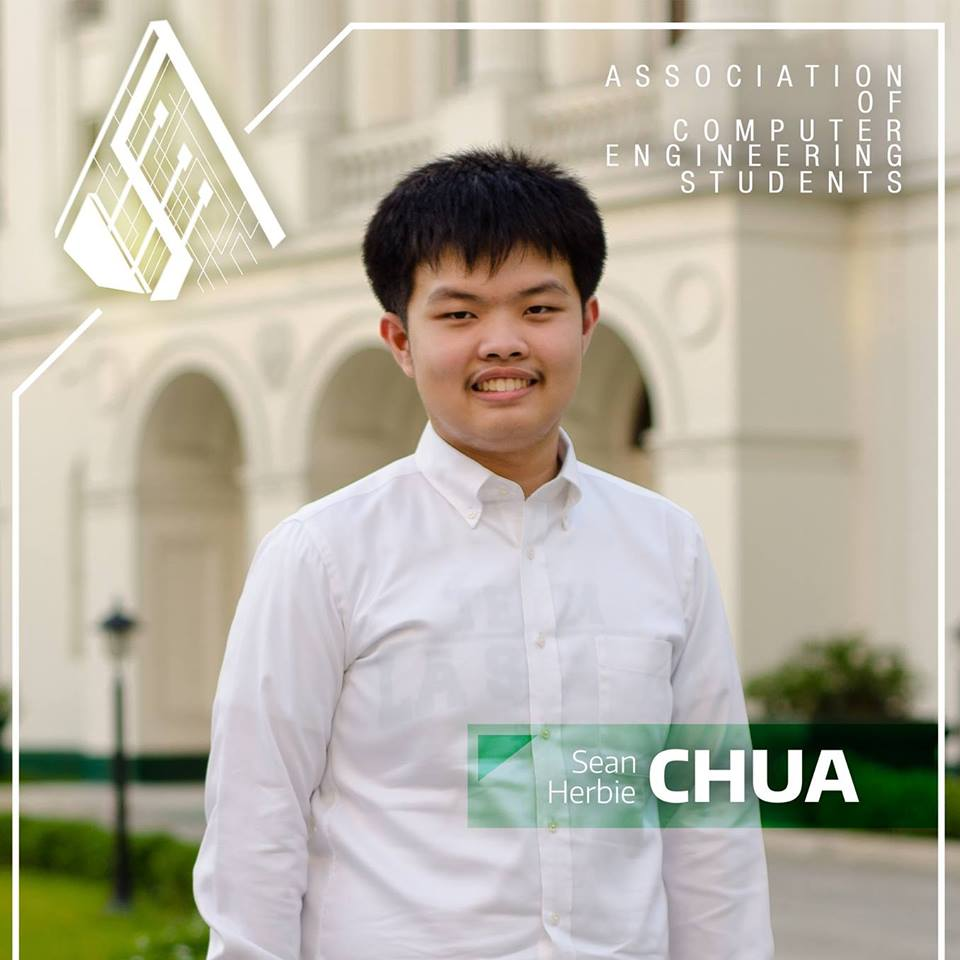
\includegraphics[width=0.2\columnwidth]{author1}
\documentAuthor{firstname1} \ \documentAuthor{surname1} \ took his primary and secondary education in Grace Christian College. He is currently taking up Bachelor of Science in \degree \ in De La Salle University. He has programmed several applications, C programming, Java programming, and Android programming. He also has a background on PIC programming. In his previous courses, he and his teammates have created a wall follower mobile robot. His interest is creating new innovations and upgrading current technology to simplify tasks.

% received the B.Sc., M.Sc., and Ph.D. degrees in chemistry all from the Pamantasan ng Pilipinas, San~Juan, Metro~Manila, Philippines, in {\xinttheiexpr \xintexpr \the\year - 5 \relax \relax}, {\xinttheiexpr \xintexpr \the\year - 3 \relax \relax} and \the\year \ respectively. He is currently taking up his B.Sc. \degree \ studies.  He has developed several high-speed packet-switched network systems and node modules. His research interests include high-speed packet-switched networks, high speed radio interface design, discrete simulation and statistical models for packet switches.

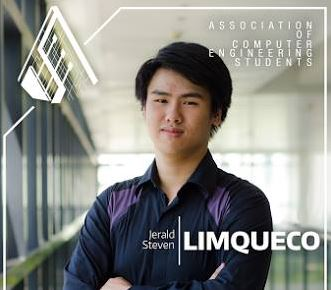
\includegraphics[width=0.2\columnwidth]{author2}
\documentAuthor{firstname2} \ \documentAuthor{surname2} \ is a third year engineering student taking up B.Sc. \degree \ at De La Salle University. He has designed and programmed several electronic circuits using Arduino and PIC as microcontrollers in some of his previous projects. He has also programmed several applications using java and C language. His research interests include environmental friendly gadgets, mobile robots that can help the society and agricultural technologies.

% received the B.Sc., M.Sc., and Ph.D. degrees in chemistry all from the Pamantasan ng Pilipinas, San~Juan, Metro~Manila, Philippines, in {\xinttheiexpr \xintexpr \the\year - 5 \relax \relax}, {\xinttheiexpr \xintexpr \the\year - 3 \relax \relax} and \the\year \ respectively. He is currently taking up his B.Sc. \degree \ studies.  He has developed several high-speed packet-switched network systems and node modules. His research interests include high-speed packet-switched networks, high speed radio interface design, discrete simulation and statistical models for packet switches.

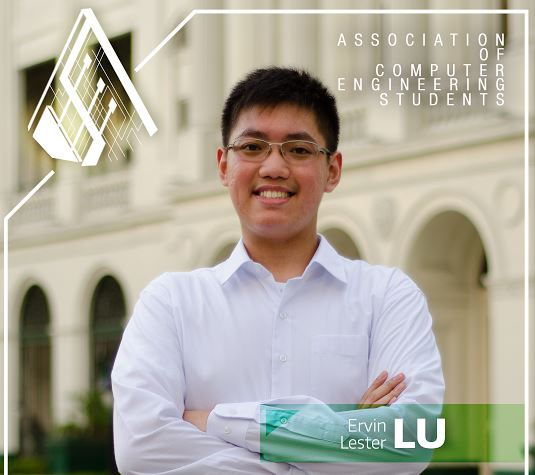
\includegraphics[width=0.2\columnwidth]{author3}
\documentAuthor{firstname3} \ \documentAuthor{surname3} \ is a third year engineering student taking up B.Sc. \degree \ at De La Salle University. He has designed and programmed several mobile applications and electronic circuits. He also has experienced using Arduino and PIC as microcontrollers in some of his previous projects. His research interests include educational mobile applications, environmental friendly gadgets, and agriculture technologies.

% received the B.Sc., M.Sc., and Ph.D. degrees in chemistry all from the Pamantasan ng Pilipinas, San~Juan, Metro~Manila, Philippines, in {\xinttheiexpr \xintexpr \the\year - 5 \relax \relax}, {\xinttheiexpr \xintexpr \the\year - 3 \relax \relax} and \the\year \ respectively. He is currently taking up his B.Sc. \degree \ studies.  He has developed several high-speed packet-switched network systems and node modules. His research interests include high-speed packet-switched networks, high speed radio interface design, discrete simulation and statistical models for packet switches.

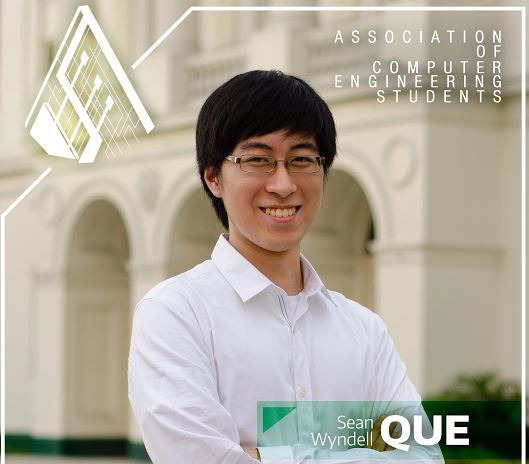
\includegraphics[width=0.2\columnwidth]{author4}
\documentAuthor{firstname4} \ \documentAuthor{surname4} \ is a third year engineering student taking up B.Sc. \degree \ at De La Salle University. He has designed and programmed several electronic circuits using PIC microcontrollers and mobile appliations using C and Java languages. His research interests include cool electronic gadgets and awesome mobile appliations.
% received the B.Sc., M.Sc., and Ph.D. degrees in chemistry all from the Pamantasan ng Pilipinas, San~Juan, Metro~Manila, Philippines, in {\xinttheiexpr \xintexpr \the\year - 5 \relax \relax}, {\xinttheiexpr \xintexpr \the\year - 3 \relax \relax} and \the\year \ respectively. He is currently taking up his B.Sc. \degree \ studies.  He has developed several high-speed packet-switched network systems and node modules. His research interests include high-speed packet-switched networks, high speed radio interface design, discrete simulation and statistical models for packet switches.

\vfill
% }